\documentclass[a4paper,man,natbib,floatsintext,noextraspace]{apa6}

\usepackage[english]{babel}
\usepackage[utf8x]{inputenc}
\usepackage{amsmath}
\usepackage{graphicx}
\usepackage[colorinlistoftodos]{todonotes}
\usepackage{apacite}

\title{Development of affordance perception and recalibration}
\shorttitle{Affordance Perception and Recalibration}
\author{John M. Franchak}
\affiliation{University of California, Riverside}

\abstract{250 words, doesn't count towards word count}

\begin{document}
\maketitle

\section{Introduction}

Perceiving affordances means distinguishing which actions are possible given the body's size and capabilities \citep{Gibson79}. For example, the affordance for passing through a narrow doorway may be possible for a small child but impossible for a large adult. If perception is \textit{calibrated}---meaning that affordance perception is correctly scaled to the body's abilities---the child would perceive the doorway as possible to navigate but the adult would not. However, uncalibrated perception may lead the observer to make a poor decision, such as attempting to fit through a doorway that is too small or refusing the walk through a doorway that is sufficiently large. Developmental studies suggest that affordance perception becomes better calibrated through childhood. Younger children (3-5 years) make large errors when choosing whether to reach through openings of varying size, but by 7 years children’s perception is calibrated as well as adults' \citep{ChildReaching}. Similarly, children aged 4-5 grossly misjudge whether inclined surfaces are possible to stand on \citep{KlevbergAnderson} and 6- and 8-year-olds overestimate their abilities to reach, step, and duck under barriers \citep{Plumert95} compared with adults.

Affordances continually change. Over development, new and improved motor skills alter abilities, as does physical growth. In the short term, carrying or using objects can temporarily alter abilities. For example, wearing a backpack increases the doorway size needed for passage \maskcitep{Recal,DoorwayLearning} and wearing platform shoes allows actors to sit on higher seats \citep{Mark87}. However, altered affordances lead to perception becoming uncalibrated because actions that were once possible may no longer be. Adults can \textit{recalibrate} their affordance perception to reflect changes in the body and abilities if they can access the right perceptual information \citep{Recal,DoorwayLearning,Mark87,MarkSitting90}. 

How does the ability to recalibrate to changing affordances develop? Whereas numerous studies have investigated children's perception of their unaltered abilities, only a handful have tested children's ability to recalibrate. One study investigated 11-year-old children’s judgments of reaching while adapting to different levels of postural support \citep{JohnsonWade2009}. Children updated judgments with respect to changing postural conditions; however, actual affordances were not measured in the altered conditions, rendering it impossible to say how successfully children recalibrated. This was addressed in a study of adapting to changes in sitting ability when wearing platform shoes: Results suggested that children might have adult-like abilities to recalibrate by 12 years \citep{ChenRecal}. Notably, children's perception of their altered abilities were as well-calibrated by the end of the study as their original, unaltered abilities, suggesting that children fully recalibrated. However, we lack a comprehensive understanding of children's abilities to recalibrate to changing affordances because prior work has studied only two different affordances, reaching and sitting, and has only tested children in a single age group (11-12 years). 

The current study expands on past work by comparing younger children (4-7 years), older children (8-11 years) and adults in a different task---squeezing through doorways with or without a backpack that alters body size. The process of recalibration varies for different affordances \citep{Recal}. In particular, recalibration in the sitting height task used by \cite{ChenRecal} is accomplished gradually over time from movement experience \cite{Mark87}. \textit{Practice feedback} from actually sitting on seats---performing the action and observing the results---is not required for recalibration in the sitting task \citep{MarkSitting90}. However, practice feedback is required to recalibrate to altered body size in the doorway squeezing task \citep{Recal,PregAps}. In particular, adults' recalibration in the squeezing task depends on receiving both success feedback (i.e., fitting through a sufficiently large doorway) and failure feedback (i.e., attempting to fit through a small doorway and becoming stuck) \citep{DoorwayLearning}. Because the squeezing task depends on participants generating feedback by practicing, cautious participants who never attempt to fit through small doorways (which would provide failure experience) will not recalibrate successfully. Indeed, a recent study that tested adults in the squeezing task and allowed them to practice as much or as little as they wished found that adults rarely chose to practice; consequently, adults did not recalibrate as fully compared with a condition when they were forced to practice squeezing through doorways \citep{DoorwayExplore}. 

The role of practice feedback may depend on age-related changes in risk taking. Whereas adults tend to be cautious and avoid practicing fitting into small doorways \citep{DoorwayExplore}, toddlers are at the other extreme: 17-month-olds attempted to wedge themselves into impossibly small doorway trial after trial \citep{InfantAps}. However, toddlers did not become better calibrated despite repeated practice, suggesting that they do not effectively learn from feedback \citep[see also][]{JohAdolph2006}. Thus, risky infants get lots of feedback but cannot learn from it, whereas cautious adults do learn from feedback but do not generate enough of it. Children make riskier decisions compared with adults across a variety of motor tasks \citep{ChildReaching, DekkerNardini, Plumert95}, and more active and undercontrolled temperament predicts individual differences children's risk taking \citep{Plumert97}. Thus, compared with adults, children are predicted to more often choose to practice squeezing through impossibly small doorways, which will provide children with feedback necessary for recalibration. 

Whether children can effectively recalibrate using practice feedback is an open question. There are two competing hypotheses. One on hand, because children experience more change to their bodies and abilities on a regular basis they might be better at recalibration compared with adults, whose bodies and abilities change less frequently. On the other hand, recalibration might be a complex skill that is more difficult for children compared with work. Related work on motor adaptation---that is, adjusting movements patterns to deal with perturbations---shows mixed results regarding infants and children's adaptation ability. One study found that infants quickly adapted their gait patterns to compensate with wearing a platform shoe on one foot that disrupted the gait cycle \citep{ColeGill2014}, but adults did not compensate. In contrast, children under 11 years of age struggled to adapt to walking on a split-belt treadmill that required learning a new way to coordinate the timing of steps \cite{Vasudevan2011}, suggesting that adults' ability to adapt is superior to children's.  

Thus, the current study asked how effectively younger children (4-7 years), older children (8-11 years), and adults recalibrate using practice feedback in the doorway squeezing task. In a block of \textit{decision trials}, participants judged whether they could squeeze through doorways that varied in width. If they judged a doorway to be possible, they attempted to walk through which provided practice feedback. \textit{Judgment accuracy} and \textit{judgment bias} were compared between participants in the \textit{original abilities} condition (OA), whose bodies were not altered, and participants in the \textit{manipulated abilities} condition (MA), who wore a backpack and thus needed to recalibrate their judgments. Accuracy was measured by magnitude of error---how much the doorways that participants attempted differed from their actual abilities. Bias was determined by measuring the direction of errors---whether participants tended to err by attempting risky, impossible doorways versus avoiding large, possible doorways. Because prior work showed that recalibration in the squeezing task depended on experiencing both success and failure feedback \citep{DoorwayLearning}, accuracy was compared between participants who received both success and failure feedback (informative feedback) and those who did not (uninformative feedback).

\section{Method}

\subsection{Participants and design}

A total of 104 participants in three age groups completed the experiment: 4- to 7-year old younger children ($M$ age = 5.5 years, $SD$ = 0.84, \textit{n} = 40, 19 female), 8- to 11-year-old older children ($M$ age = 9.5 years, \textit{SD} = 0.84, \textit{n} = 40, 22 female), and college-aged adults ($M$ age = 18.9 years, \textit{SD} = 2.2, \textit{n} = 24, 13 female). Half of the participants from each age group were assigned to either the original ability (OA) condition or the manipulated ability (MA) condition in a fully between-subjects design. Two MA participants (1 younger children and 1 older child) were excluded due to computer issues in recording the data, resulting in a final sample of \textit{N} = 102. Four additional children were recruited but failed to complete both blocks of trials. 

Families were recruited from local community events and Internet advertisements. Families were compensated \$10 for their participation and children received a small toy or book. Adult participants were recruited through the psychology department subject pool to fulfill a course requirement. Participants reported their ethnicity as Hispanic (42.3\%) or non-Hispanic (52.9\%); 3.9\% declined to respond. Participants identified their race as White (46.1\%), more than one race (21.6\%), other (15.7\%), Asian (6.8\%), Black or African American (3.9\%), and American Indian or Alaskan Native (2.9\%); 2.9\% declined to respond.

\subsection{Apparatus}

An adjustable doorway apparatus was used as in prior work \citep{DoorwayLearning,Recal}. A free-standing steel frame supported a stationary wall (182 cm tall × 62 cm wide) and an overhead track. A sliding wall (185 cm tall × 100 cm wide) moved along the track (perpendicular to the stationary wall) to create doorways varying in width from 0 to 70 cm. A measurement camera attached to the sliding wall recorded calibration markings that were used by the experimenter to adjust the doorway size in 0.5 cm increments. The sliding wall had a locking mechanism that, while engaged, kept the doorway at a fixed width while the participant squeezed through. A video camera recorded a side view of the participant’s approach and passage through the doorway for later coding.

Participants in the manipulated ability condition wore a backpack that measured 35 cm tall × 25 cm wide × 12 cm deep and weighed 1 kg on their backs to increase body size and thus alter doorway fitting ability. The backpack was filled with rigid cardboard so that it did not compress while participants squeezed through the doorway. 

\subsection{Procedure}

The experiment consisted a block of 35 decision trials followed by a block of 10 ability trials. Decision trials assessed participants’ judgments of whether they were able to squeeze through doorways and provided practice feedback when participants attempted to walk through doorways they deemed possible. Ability trials verified which doorways participants could successfully squeeze through to determine error. MA participants put on the backpack at the beginning of the session and wore it during both blocks of trials; OA participants did not wear the backpack. The entire session lasted approximately 45 minutes. 

\subsubsection{Decision trials}

Participants began each decision trial facing away from the doorway at a starting line 320 cm away. Once the experimenter set the doorway to the correct width, an assistant standing near the starting line told the participant to turn around and asked, “Do you think you can squeeze through that doorway without getting stuck?”. Participants’ yes/no responses were recorded and then later verified from video. If the participant replied “yes”, the assistant instructed the participant to try to squeeze through. The experimenter scored whether the participant successfully squeezed through the doorway (touching the sides of the doorway was allowed) or failed by becoming stuck; online success/failure outcomes were later verified from video. If the participant replied “no”, the assistant instructed the participant to turn back around to wait for the next trial.

The decision trial block started with two warm-up trials to familiarize participants with the task by presenting a clearly possible doorway (40 cm) followed by a clearly impossible doorway (4 cm). Afterwards, participants completed 33 trials composed of 3 sets of 11 predetermined doorway widths based on age and condition (see below); each set was presented in a randomized order. Doorway widths were selected based on pilot testing and past work \citep{Recal} to ensure that each participant was exposed to both possible and impossible doorway widths depending on their body size and whether they wore the backpack. For the original ability condition, younger and older children were presented with doorways 6-26 cm in 2-cm increments (i.e., 6, 8, 10, 12, 14, 16, 18, 20, 22, 24, and 26) and adults were presented with doorways 10-30 cm. Doorway sizes in the MA condition were 12-32 cm for younger and older children and 16-36 cm for adults. 

\subsubsection{Ability trials}

For each ability trial, the experimenter set the doorway to a particular size and then the assistant instructed the participant to attempt to fit through, “I want you to try to fit through the doorway even if you don’t think you can. If you get stuck it’s OK”. The experimenter scored whether the participant successfully squeezed through the doorway or failed by becoming stuck; online scores were later verified from video. On the first ability trial, the doorway was set to the median doorway size presented during the decision trial block (for example, a child in the original ability condition started with a 16-cm doorway). Each successive trial was determined using a staircase procedure: The doorway size was decreased by 2 cm following a successful attempt and was increased by 1.5 cm following a failed attempt.

\subsubsection{Data analysis}

The goal of data analysis was to determine the accuracy and bias of decisions by comparing decision data to ability data. As in past work \citep{Recal,PregAps}, cumulative Gaussian functions were fit to decision data (proportion “yes” responses at each doorway width) and ability data (proportion successful passage at each doorway width). Decision functions used only trials from the decision trial block; ability functions used “yes” trials from the decision trial block (in which participants attempted to pass through the doorway) in addition to ability trials. Maximum likelihood fits for the threshold of each function were calculated using the Palamedes toolbox \citep{KingdomPrins} in Matlab. Parametric bootstraps with 1000 Monte Carlo iterations determined 95\% confidence intervals for threshold parameters. 

Decision thresholds reflected the doorway width that participants judged to be possible to fit through 50\% of the time. Decision thresholds were fit well for each age based on relatively small confidence intervals for younger children ($M$ = 18.9 cm ± 1.62), older children ($M$ = 20.6 cm ± 1.54), and adults ($M$ = 24.3 cm ± 1.14). Although confidence intervals appeared to be marginally smaller for adults, confidence interval size did not differ by age group in a one-way ANOVA ($p$ = .09). Ability thresholds indicated the doorway width that participants successfully fit through 50\% of the time. Small confidence intervals around ability threshold estimates for younger children ($M$ = 17.6 cm ± 0.58), older children ($M$ = 19.3 cm ± 0.54), and adults ($M$ = 23.8 cm ± 0.40) indicate good fits. Confidence interval size did not differ by age group in a one-way ANOVA ($p$ = .65).

For a small subset of participants, decision functions could not be fit because participants either replied “yes” to every doorway (1 younger child in the OA condition) or “no” to every doorway (1 younger child, 4 older children, and 2 adults in the MA condition). For the participant who said “yes” to every doorway, the decision threshold was set 2 cm smaller than the smallest doorway presented in the decision trial block. For the participants who said “no” to every doorway, decision thresholds were set 2 cm larger than the largest doorways they received in the decision trial block. This approximation assumes that if participants received the next 2-cm increment beyond the testing range that their decisions would have changed. This approximation is conservative and likely underestimates the magnitude of these participants’ errors because a change in doorway size > 2 cm might have been required for participants to change their decisions. 

\section{Results}

Judgment accuracy and bias were calculated based on decision and ability thresholds. Accuracy was indexed by \textit{absolute judgment error}---the magnitude of errors regardless of direction---and was calculated as the absolute value of the difference between decision and ability thresholds. \textit{Constant error} represented judgment bias in participants’ errors and was calculated by subtracting ability thresholds from decision thresholds. Absolute errors were not distributed normally because they were bounded at 0. Additionally, preliminary analyses revealed significant Levene’s tests for homogeneity of variance when testing both absolute and constant error by condition and age group. Thus, non-parametric permutation ANOVAs and t-tests were used because they do not require those assumptions \citep{Edgington}. Permutation tests were conducted in R using the \textit{ez} and \textit{rcompanion} packages using 1000 iterations. Effect size estimates (generalized $\eta^{2}$) were derived from parametric ANOVAs calculated using the \textit{ez} package. $p$ values in follow-up tests were adjusted for multiple comparisons with the Holm-Bonferroni correction.

\subsection{Judgment accuracy}

Figure \ref{fig:error}A shows that absolute errors decreased with age for the OA condition but not the MA condition and that errors were larger overall in the MA condition compared to the OA condition. A 3 Age (younger children, older children, adults) × 2 Condition (OA, MA) permutation ANOVA yielded a significant age effect ($p = .012, \eta^{2} = .10$), a significant condition effect ($p < .001, \eta^{2} = .10$), and a significant age × condition interaction ($p = .023, \eta^{2} = .08$). To follow-up on the interaction, pairwise comparisons of error by age were conducted separately for each condition. In the OA condition, permutation t-tests confirmed that errors decreased with age (all groups differed significantly, $p$s < .02): Younger children made larger errors ($M$ = 4.15 cm, $SD = 2.65$) compared with older children ($M$ = 2.01 cm, $SD = 1.34$), and older children's errors were larger than adults' ($M$ = 1.00 cm, $SD = 0.65$). In contrast, absolute errors in the MA condition for younger children ($M$ = 4.11 cm, $SD = 2.51$), older children ($M$ = 5.24 cm, $SD$ = 3.87), and adults ($M$ = 3.03 cm, $SD = 2.75$) did not significantly differ (permutation t-tests $p$s > .29). A second set of pairwise comparisons tested for condition effects within each age group. Whereas younger children performed similarly regardless of condition ($p = .96$), older children ($p = .006$) and adults ($p = .048$) were less accurate when recalibration was required in the MA condition.

\begin{figure}[htb!]
\centering
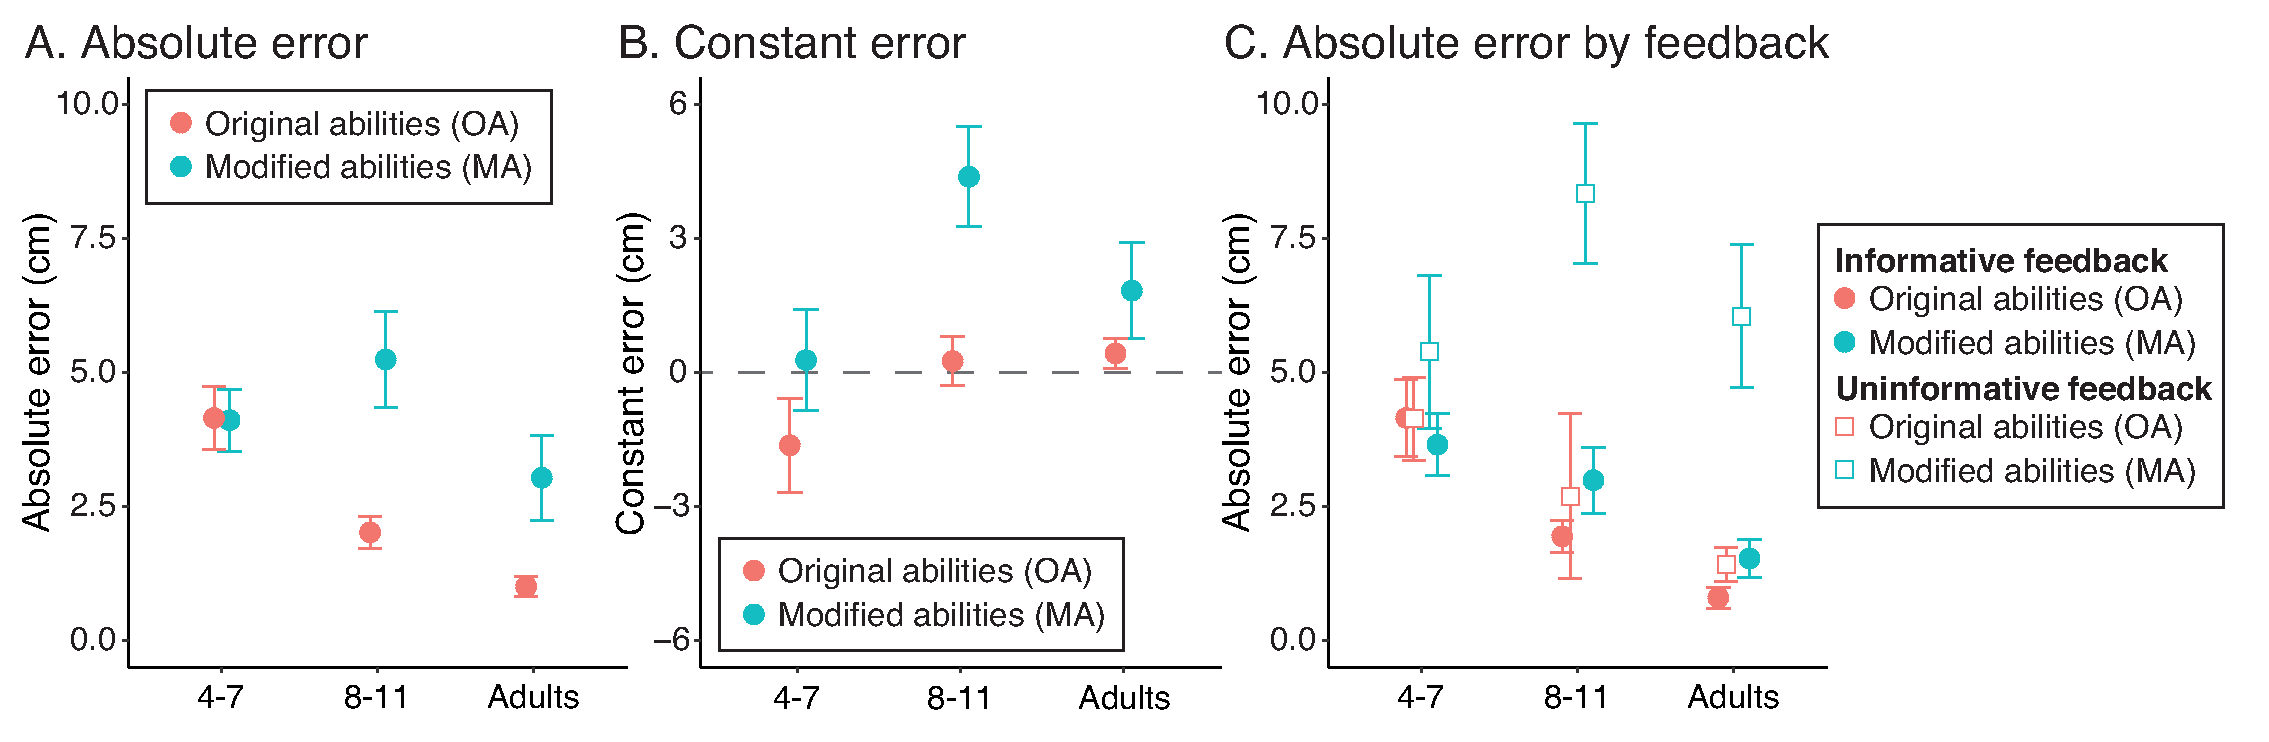
\includegraphics[width=1\textwidth]{error.eps}
\caption{\label{fig:error}(A) Absolute error and (B) constant error by age group and condition. Red symbols show the original ability condition and blue symbols show the modified abilities condition. (C) Absolute error by age group, condition, and feedback group. Circular symbols depict the informative feedback group and square symbols show the uninformative feedback group. Error bars show ± 1 SE.}
\end{figure}

\subsection{Judgment bias}

Figure \ref{fig:error}B shows that constant error increased with age and was greater for the MA condition compared with the OA condition. In the OA condition, younger children were riskier and biased towards selecting impossibly small doorways ($M$ = -1.63 cm, $SD = 4.72$); older children ($M$ = 0.25 cm, $SD$ = 2.45) and adults ($M$ = 0.42 cm, $SD$ = 1.14) were relatively unbiased---neither cautious nor risky. In the MA condition, more conservative judgments overall meant that younger children were unbiased ($M$ = 0.27 cm, $SD$ = 4.90) and that older children ($M$ = 4.38 cm, $SD$ = 4.87) and adults ($M$ = 1.82 cm, SD = 3.73) were more cautious and often said “no” to doorways that were indeed possible to fit through. A 3 Age (younger children, older children, adults) × 2 Condition (OA, MA) permutation ANOVA confirmed significant main effects of age ($p = .014, \eta^{2} = .10$) and condition ($p < .001, \eta^{2} = .09$), but the interaction was non-significant ($p = .35, \eta^{2} = .02$). The main effect of age was followed up by comparing each age group while collapsing across conditions. Younger children were significantly riskier compared to older children as evidenced by smaller constant errors ($p$ = .006); however, no significant differences were found between younger children and adults ($p$ = .19) or between younger children and adults ($p$ = .25).

\subsection{Feedback and judgment accuracy}

Participants were grouped based on feedback experiences during the decision trial block. The informative feedback (IF) group contained participants who experienced both success and failure feedback during the decision trial block, whereas the uninformative feedback (UF) group contained participants who received only success feedback, only failure feedback, or no feedback during the decision trial block (Table \ref{tab:1}). 

\begin{table}
\caption{Absolute error (M and SD) and group size for participants in the informative feedback (IF) and uninformative feedback (UF) groups by age and condition.}
\label{tab:1}
\begin{tabular}{@{}lllllllll@{}}
\multicolumn{4}{c}{Informative Feedback (IF)}                                                                                   &                       & \multicolumn{4}{c}{Uninformative Feedback (IF)}                                                                  \\ 
\multicolumn{1}{l}{Condition} & \multicolumn{1}{l}{Age} & \multicolumn{1}{l}{\textit{M (SD)}} & \multicolumn{1}{l}{\textit{n}} & \multicolumn{1}{l}{} & \multicolumn{1}{l}{Condition} & \multicolumn{1}{l}{Age} & \multicolumn{1}{l}{\textit{M (SD)}} & \multicolumn{1}{l}{$n$} \\ \midrule
OA                              & 4-7                      & 4.1 (2.9)                            & 16                              &                       & OA                             & 4-7                      & 4.1 (1.6)                   & 4                      \\
OA                              & 8-11                     & 1.9 (1.3)                            & 18                              &                       & OA                             & 8-11                     & 2.7 (2.2)                   & 2                      \\
OA                              & Adults                   & 0.8 (0.5)                            & 8                               &                       & OA                             & Adults                   & 1.4 (0.6)                   & 4                      \\
MA                              & 4-7                      & 3.7 (2.2)                            & 14                              &                       & MA                             & 4-7                      & 5.4 (3.2)                   & 5                      \\
MA                              & 8-11                     & 3.0 (2.0)                            & 11                              &                       & MA                             & 8-11                     & 8.3 (3.7)                   & 8                      \\
MA                              & Adults                   & 1.5 (1.0)                            & 8                               &                       & MA                             & Adults                   & 6.0 (2.7)                   & 4                      \\ \bottomrule
\end{tabular}
\end{table}

Figure \ref{fig:error}C shows absolute error as a function of age, condition, and feedback type and reveals two striking results. First, only participants who received uninformative feedback struggled to recalibrate to modified abilities; there was no difference between MA and OA conditions for IF participants. Second, in the MA condition accuracy improved for IF participants, suggesting that the ability to recalibrate using feedback improve with age when considering only those participants who received the required feedback. These results were confirmed in a 3 Age (younger children, older children, adults) × 2 Condition (OA, MA) × 2 Feedback (IF, UF) permutation ANOVA on absolute error. As before (when feedback was not included in the model), the ANOVA revealed significant main effects of age ($p = .006, \eta^{2} = .10$) and condition ($p < .001, \eta^{2} = .15$) as well as a significant age × condition interaction ($p = .034, \eta^{2} = .06$). Furthermore, adding feedback to the model resulted in a significant feedback effect ($p < .001, \eta^{2} = .15$) and a significant condition feedback interaction ($p = .001, \eta^{2} = .10$). No other effects reached significance. 

To follow up on the age × condition and feedback × condition interactions, data were split by feedback group to run two separate 3 Age × 2 Condition permutation ANOVAs. For participants who generated informative feedback, the 3 Age × 2 Condition ANOVA revealed only a significant effect of age ($p < .001, \eta^{2} = .24$)---as Figure \ref{fig:error}C shows, the lines for the OA and MA conditions are superimposed and both decrease with age. Pairwise comparisons between age groups (collapsed across condition) confirmed that absolute error significantly differed between all three groups ($p$s < .016). In contrast, participants who experienced uninformative feedback showed a completely different pattern of results. The 3 Age × 2 Condition ANOVA revealed only a significant effect of condition ($p = .006, \eta^{2} = .33$, which indicates that although participants' perception of their original affordances were well-calibrated regardless of feedback, recalibration to altered affordances depended on feedback for all three age groups.

\section{Discussion}

The current study examined how young children, older children, and adults recalibrate to changing affordances for squeezing through doorways. Two groups were compared: Participants who judged their original, unmodified affordances and participants who recalibrated to wearing a backpack that altered affordances for fitting through doorways. The results replicated previous work that showed age-related changes in affordance perception for unmodified abilities as well as risk-taking behavior in motor tasks, but extended past work by using a previously unstudied task (squeezing through doorways). More important, the results of the current study are novel in showing age-related changes in children's ability to recalibrate to altered affordances using feedback information.

As in past work \citep{Plumert95,ChildReaching,KlevbergAnderson}, children's perception of affordances for their unmodified abilities improved with age. In the OA condition, younger children (4-7 years) made larger errors compared with the older children (8-11 years), and older children made larger errors compared with adults. Taken together with previous work, findings are mixed regarding the age at which calibration of affordance perception becomes adult-like. Whereas 7-year-olds' judgments about reaching through openings were as accurate as adults' \citep{ChildReaching}, children aged 8-11 in the current study and in \cite{Plumert95} made larger errors compared with adults in other tasks. Most likely, age-related changes in affordance perception vary according to task; mature calibration in one task should not imply mature calibration in other tasks. 

The current study's findings are also consistent with past work showing age-related changes in risk-taking behavior in motor tasks \citep{Plumert95,DekkerNardini,Plumert97}. Across conditions, younger children were more likely to attempt to squeeze through impossibly small doorways compared with older participants. Unlike past work that found younger and older children to be equally risky \citep{DekkerNardini}, the current study found that older children were more cautious compared to younger children and equally cautious as adults. Across ages, participants' bias differed by condition. Participants judging their unaltered abilities were more risky compared to those who recalibrated to wearing the backpack. Caution when recalibrating could reflect participants' uncertainty or a lack of confidence when adapting to altered abilities. A second possibility is that participants expect the backpack to alter their abilities by a greater degree than it actually did; other work using the squeezing task found that adults made cautious judgments while wearing a "pregnancy pack" \citep{PregAps}. Although the pregnancy pack added 15 cm to participants' bodies, because it compressed while participant squeezed through doorways it added only 10 cm to their ability thresholds. The degree to which the backpack compressed could not be assessed in the current study because ability thresholds without the backpack for were not measured for participants in the MA condition.

The primary aim of the current study was to determine how effectively children recalibrate to altered affordances---does frequent change in body size and abilities confer a benefit to children when recalibrating or is recalibration a difficult skill that children need to master? At first glance, the overall analysis of absolute error appeared to indicate that participants of all ages struggled in the recalibration task: Errors in the MA condition were larger compared to those in the OA condition, indicating that participants were better calibrated when judging their unaltered abilities compared to when recalibration was necessary. However, previous studies using the doorway squeezing task show that participants' ability to recalibrate depends on informative feedback---experiencing both successful and failed practice attempts \citep{DoorwayExplore, Recal}. Thus, it would be unreasonable to expect that participants who received uninformative feedback would recalibrate successfully. Indeed, participants who received uninformative feedback made inaccurate judgments in the MA condition regardless of age. \todo{Something about different access to feedback related to caution?}

Errors decreased with age in the MA condition when examining only those participants who received informative feedback. Thus, with age participants became more effective at recalibrating from practice feedback. Past work found adult-like recalibration for 12-year-olds in the sitting task \citep{ChenRecal}, however, even the oldest children in the squeezing task lagged behind adults in the squeezing. The discrepancy between the tasks suggests that recalibrating using different types of information (i.e., movement experience in the sitting task, practice feedback in the squeezing task) might develop differently. Furthermore, although older children were adult-like when judging altered abilities, they struggled in comparison to adults when recalibrating. Taken together, these points reaffirm the need to study the development of affordance perception and recalibration across a wider set of tasks. 

\todo{Conclusion?}

\bibliography{example}

\end{document}

